% =========================================================
% intro.tex
% =========================================================
% The introduction to the final project

\section*{Introduction}

With the increasing reliance on digital systems in the
modern age, maintaining the security and privacy of
important data is more critical than ever. As such,
cryptographic algorithms for securly storing and
communicating data have widespread usage. To maintain
security, these algorithms are centered around
computational problems that are infeasible for classical
processors to solve; these are known as \textit{NP-hard}
problems, which have no known polynomial time solution.
Users with a secret key are able to decrypt the encoded
messages, but users without would have to solve this
NP-hard problem to access the encrypted data, which are
designed to take an astronomical number of years to solve
with brute-force.

The advent of quantum computers have called the stengths of
many of these algorithms into question. For example, both
RSA (a popular asymmetric-key algorithm with widespread
use) and Diffie-Hellman (an algorithm for securly
establishing a common shared key, for use in symmetric-key
encryption) rely on the difficulty of factoring large
numbers for their security. Algorithms for quantum
computers to solve such problems in polynomial time have
existed for a while \cite{shor}, but have never had a
computer advanced enough to run them. However, modern
advances in quantum computing have demonstrated that
computers may be available soon that can crack these
algorithms. Even just earlier this week, Google unveiled
a new quantum computer, "Willow", that can achieve
speedups over the fastest classical processors on select
problems by a factor of $10^{30}$ \cite{willow}.

\begin{wrapfigure}{r}{0.35\textwidth}
  \centering
  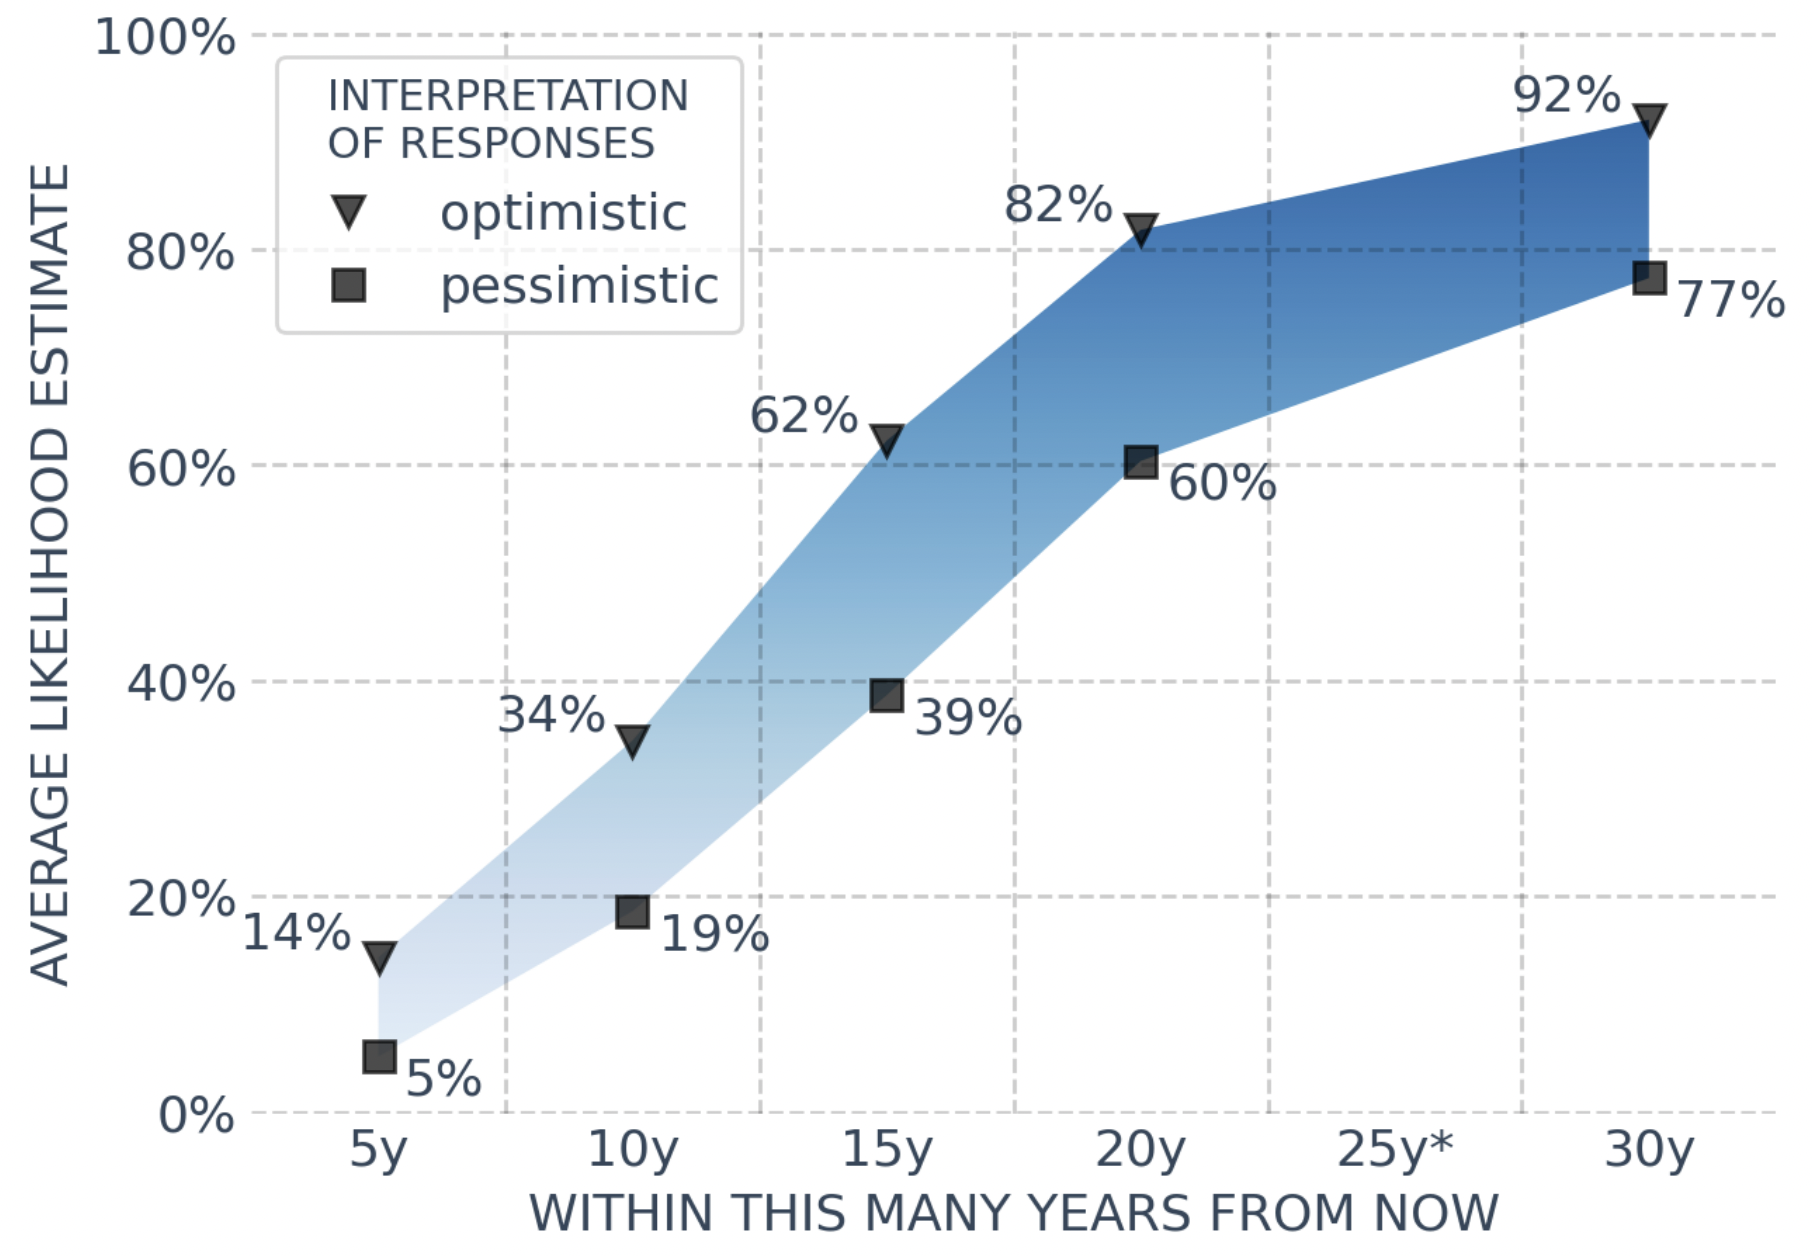
\includegraphics[width=\linewidth]{imgs/intro-timeline.png}
  \caption{
    A timeline of when experts believe that RSA-2048 will be
    able to be broken by a quantum computer in 24 hours
    \cite{threat-report}}
  \label{fig:intro-timeline}
\end{wrapfigure}

While such computers aren't currently able to break modern
cryptographic algorithms, many experts suspect it's only a
matter of time before current cryptographic algorithms
become insecure \cite{threat-report}. To this end, NIST
(the National Institute of Standards and Technology)
has standardized the use of RSA-2048 only until 2030, and
noted that updated strengths are heavily affected by any
progress on quantum computing \cite{nist-standards}.
Additionally, to prepare for the advance of quantum
computing, NIST has standardized additional,
\textit{quantum-resistant} algorithms \cite{nist-kyber}.
These algorithms are centered around different
computational problems for which there is no known
algorithm to efficiently solve for both classical and
quantum computers. This \textit{post-quantum cryptography}
(PQC) will have increasing significance as advances in
quantum computers are made. Additionally, since malicious
adversaries could already be recording data to later
decrypt once sufficient quantum computers are available,
PQC algorithms are already being recommended and used for
extremely sensitive data, such as government operations
\cite{quantum-law}.

For public-key encryption (where the encrypting and
decrypting keys are different), as well as key
establishment (for securely establishing a shared secret
key over an insecure network), NIST recommends
CRYSTALS-Kyber, or simply \textbf{Kyber}. Since such an
algorithm would be widely used in communication, speeding
up its operation would have large impacts for a variety of
applications. For our project, we explored implementing
Kyber using custom hardware on an FPGA.